% simple.tex -- Yaser Alkayale Thesis Taken From Vlado Keslj

\documentclass[12pt]{dalthesis}

\usepackage[algochapter,ruled,vlined,longend,linesnumbered,resetcount]{algorithm2e}
\usepackage{mathtools}
\usepackage[T1]{fontenc}
\usepackage{siunitx}
\usepackage{tikz} % To generate the plot from csv
\usepackage{pgfplots}
\usepackage{filecontents}
\usepackage{graphicx}
\usepackage{amsmath}
\usepackage{subcaption}
\usepackage{siunitx}
\usepackage{natbib}
\usepackage{amssymb}
\usepackage{hyperref}


\hypersetup{
    colorlinks=true,
    linkcolor=blue,
    filecolor=blue,      
    urlcolor=blue,
    citecolor=blue,
    pdftitle={Yaser Alkayale Thesis}
}
\urlstyle{same}


\captionsetup{compatibility=false}

\newcommand*{\Value}{\frac{1}{2}x^2}
\newcommand*{\kmeansn}{\textsc{K-Means}} %kmeans with no space
\newcommand*{\kmeans}{\kmeansn } %kmeans with space

\usepgfplotslibrary{external}
\tikzexternalize{yaser_thesis}
\pgfplotsset{compat=newest} % Allows to place the legend below plot
% \usepgfplotslibrary{units} % Allows to enter the units nicely

\sisetup{
  round-mode          = places,
  round-precision     = 2,
}

% These will help for absolute value math operators
\DeclarePairedDelimiter\abs{\lvert}{\rvert}
\DeclarePairedDelimiter\norm{\lVert}{\rVert}
\DeclareMathOperator*{\argmin}{argmin}

% This is where all the images are used.
\graphicspath{ {images/} }

\begin{document}

% Swap the definition of \abs* and \norm*, so that \abs
% and \norm resizes the size of the brackets, and the 
% starred version does not.
\makeatletter
\let\oldabs\abs
\def\abs{\@ifstar{\oldabs}{\oldabs*}}
\let\oldnorm\norm
\def\norm{\@ifstar{\oldnorm}{\oldnorm*}}
\def\BState{\State\hskip-\ALG@thistlm}
\makeatother

\title{\kmeans Clustering, An Improved Seeding Process and Novel Method to Compute the Number of Clusters for a Dataset} %TODO: Change the title.
\author{Yaser Alkayale}
\bcshon  %Sets it to honours variant
\degree{Bachelor's of Computer Science, Honours}
\degreeinitial{B.C.Sc.}
\faculty{Computer Science}
\dept{Faculty of Computer Science}
\defencemonth{April}\defenceyear{2018}
\dedicate{This thesis is in dedication to my grandfather whom I was named after.}

\nolistoftables
\nolistoffigures

\frontmatter

\begin{abstract}
  Clustering is a well-known task that has been studied and used for decades. The idea is to take a set of items and group them into a number of clusters based on a similarity measure. \kmeansn, although named differently back then, was proposed in 1957 by Stuart Lloyd and is one of the most widely used clustering algorithms and is still used today as a reasonably fast heuristic to find clusters. \kmeans has two main parts to clustering, the initial seeding process and the iteration process. The seeding process picks $k$ initial seeds as cluster centres and highly affects the accuracy of the final result in the algorithm. The iteration process moves the centres around until it converges to a local optimum. The iteration process dominates the running time. In this paper, we discuss a new method of the seeding process that promises to give us more accurate seeds to start the algorithm and a novel way to extract the underlying number of clusters in a given dataset to help \kmeans converge faster and give more accurate results.
\end{abstract}


\begin{acknowledgements}
  A sincere thank you to my supervisor Dr. Norbert Zeh. Without his assistance, this project would not have seen the light light of day. Thank you to my co-supervisor Dr. Vlado Keselj who made himself available. Also, big thank you to Arazoo who was with me from the beginning, and went through my ideas with me.
\end{acknowledgements}

\mainmatter

\chapter{Introduction \& Background}
Clustering is the task of grouping certain things into separate or overlapping groups based on a similarity criterion. Clustering problems arise in many domains such as
natural language processing \citep{ravichandran2005randomized},
bioinformatics \citep{edgar2010search}, 
crash report analysis \citep{soto2016machine},
and vehicle navigation \citep{maio1996dynamic}. 
The notion of what is a good cluster highly depends on the domain and application. Many clustering techniques like hierarchical clustering \citep{corpet1988multiple}
and graph-based clustering \citep{schaeffer2007graph}
exist. \kmeans clustering continues to be one of the most popular clustering algorithms for it's simplicity of implementation and relative efficiency \citep{jain2010data}.

Different clustering algorithms are suited for different tasks. Some of them, like \kmeansn, fit a given dataset into a given number of disjoint sets. Other algorithms allow points to belong to multiple clusters and are useful in applications such as community clustering on social media graphs \citep{epasto2017ego}. In other instances, clustering is used on datasets where the number of clusters is unknown; for example, clustering images of people using facial recognition \citep{schroff2015facenet}. The effectiveness of a given algorithm is determined by the domain it is being used in and the problem at hand.

Formally, \kmeans is the problem where one is given a set of $n$ points in $d$-dimensional space, $\mathbb{R}^d$, and a number $k$. The goal is to split the $n$ points into $k$ disjoint clusters (subsets), minimizing the cost function $\phi$, the sum of distances of each point to its cluster centre. A cluster centre is defined to be the mean of the points in the clusters. \kmeans does especially well, in terms of speed and accuracy, on convex shaped clusters as it minimizes the sum of distances of all points to their corresponding cluster centres. However, it struggles to perform well in terms of accuracy and running time when clusters are not convex shaped or $k$ is not the right number of actual clusters in the dataset. Solving \kmeans exactly is known to be NP-hard, and that is why heuristics like Lloyd's \citep{1056489} iterations were introduced to give us an approximation of the solution by using local search. A locally optimal solution is good enough in most cases, allowing us to have meaningful clusters in a reasonable amount of time.

% TODO: Add what exactly I am doing in this paper.
In this paper, we introduce a new way to seed the \kmeans algorithm. Preliminary experiments suggested that htis seeding method produced clusters of comparable quality as produced by advanced seeding strategies such as \kmeansn++ and \kmeansn||, while bing much simpler. Unfortunately, a more careful evaluation shawed that the clusters are not significantly better than those obtained using uniformly random seeds. The ideas of the algorithm and its pseudocode are outlined along with results. We also provide a C++ implementation of the algorithm and ways it can be used for further development and research.


\section{The \kmeans algorithm.}
The \kmeans algorithm is simple and relatively efficient as it minimizes the objective function locally depending on its seeds.
Here are the steps of the algorithm \citep{arthur2007k}. The input is assumed to be the dataset $X$ and the number of clusters required $k$:

\begin{enumerate}
  \item Pick $k$ arbitrary points from $X$.
  \item Point $p$ in $X$ belongs to cluster $C_i$ if $p$ is closer to $c_i$ than it is to $c_j$ for all $j \neq i$, $1 \leq i,j \leq k$
  \item For $i$ in \{1...k\} compute a new cluster centre $c_i = \frac{1}{\abs{C_i}}\sum_{x \in C_i}x$
  \item Repeat steps 2 and 3 until centres do not change\footnote{In reality, the centres rarely ever stop changing, so heuristics need to be used to stop the algorithm in reasonable time.}.
\end{enumerate}

Of course, the algorithm may not always converge in a reasonable amount of time, so a stop condition is used when the centres do not change beyond a threshold at a certain point or a limit on the number of iterations is reached.

\section{Seeding Process}

Lloyd's algorithm, sketched above, finds a locally optimal set of clusters but may fail fo find the globally optimal solution. The objective function of these two solutions may defer significantly. Hence, the choice of of the \kmeans algorithm is crucial to the accuracy of the output.
Many new approaches to pick initial seeds like \kmeansn++ \citep{arthur2007k}, and \kmeansn|| \citep{bahmani2012scalable} have been introduced which help pick seeds that converge faster, and to better local optima. Given the dataset $X$ and the number $k\leq \abs{X}$ to cluster, \kmeans picks $k$ points from the dataset uniformly at random. Lloyd's method does not specify any way of picking the initial seeds. It only required $k$ seeds to run and converge an a local optimum. The widely used method of seeding \kmeans  is to do it uniformly at random. The objective functions of the clusters computed using uniformly random seeds generally have hight variance. More robust results are obtained using more sophisticated seeding strategies. It it important to note here that mo matter the choice of seeds we are only able to compute a local optimum, not the global optimum solution because the problem is NP-hard \citep{mahajan2009planar}. 

\subsection{\kmeansn++: A Better Seeding Process}
\kmeansn++ uses an intuitive way to seed the initial clusters of the algorithm by trying to pick seeds that are as far apart as possible. This is done by giving a higher probability for points that are further away from the ones already picked. The way it works is that we pick a random initial point, and then give a higher probability of picking a point proportional to its distance from the seeds already picked, until $k$ seeds are picked \citep{arthur2007k}.

\kmeansn++ works well because by skewing the probabilities of picking seeds towards ones that are farther from the already picked ones, we are helping pick seeds in different clusters in the dataset. It works especially well because a concentration of points already has a high probability of picking at least one of them picked, and lowering the probabilities for points that are close to ones that have already been chosen allows us to probabilistically almost ensures having a point from each cluster.

\kmeansn++ works very well because it about evenly distributes the initial seeds in the dataset. It is important to note that the probabilistic model still gives a chance for any of the points to be chosen, just some higher than others. This is crucial as we are merely making ``good guesses'' as to what the initial seeds should be, but are in no way trying to compute the ``perfect seeds'' because that would be solving the \kmeans problem, and as discussed earlier, that is NP-hard.

From my research, \kmeansn++ seems to be the best scientifically proven way to seed the \kmeans algorithm. However, there have been improvements on the \kmeansn++ seeding algorithm like \kmeansn||, which improves the algorithm by making it parallelizable for very large datasets. 


\section{Iterations}

The iteration process of the \kmeans clustering algorithm dominates the running time of the algorithm. The running time for random seeding is $O(k)$, while the iterations run in $O(tnkd)$ time, where $t$ is the number of iterations.\footnote{Faster implementations of these iterations are possible using efficient data structures, but this is not the focus of this thesis.} Depending on how quickly the iterations converge, the number of iterations may be large. \kmeansn++ has a seeding cost of $O(nk^2d)$, but the cost of the iterations still dominates the running time of the algorithm for small $k$.
Different approaches have been used to run the iterations and converge the centres. These approaches have had high success in reducing the running time of the algorithm \cite{alsabti1997efficient}. However, the implementation of these methods are not as simple as Lloyd's iterations, making them not as widely used. 

\section{Objective Function}
The objective function, $\phi$, determines the set of clusters computed. The most common choice, also used in paper, is the sum of the squared Euclidean distances\footnote{Note: Here squared distance is used because comparing distances and the square maintains the ordering of the points and saves a large amount of computational time as square rooting numbers is computationally costly.}
of all the points to their cluster centres. More formally expressed as:
$$\phi = \sum_{x\in X} \min_{c\in C}\abs{ x-c}^2$$

%TODO: Check if squared distances gives the same result as regular distances.
This objective function is the reason why \kmeans inherently produces convex shaped clusters as it tries to minimize the distance of each point to its cluster centre. If a point is marginally closer to a centre than another, it is grouped with the closer one. Geometrically this disallows concave shapes of any cluster. This is good for datasets where clusters are geometrically convex or close to it, but poses problems where the underlying data is not convex or is not clearly separable.

\section{Difficulties}

\kmeans clustering is very good at clustering well-separated convex clusters where $k$ the number of clusters is known or accurately measured in advance. However, this is very rarely the case. Another issue with \kmeans is that it fits every point into a single cluster. This means that a point has no way of belonging to different clusters at the same time. 


\chapter{\kmeansn-Consensus Seeding}

Consensus seeding is a new seeding process for \kmeansn. The basic idea is to run the randomized seeding process $T$ times, followed by a small number of iterations, $S$, which produce a set of $k$ cluster centres each. We then take these ($T*K$) centres and cluster them into $k$ clusters. The resulting cluster centres are the seeds for the iteration phase of the entire dataset.


\section{The Algorithm Pseudocode}

Note: kmeans.cluster is a function that takes three values: the dataset, the number of clusters, $k$; and an optional value, the maximum number of iterations for the algorithm. The maximum number of iterations is set to infinity by default. \\

\begin{algorithm}[H]
  \caption{Consensus Seeding.}
  \SetAlgoLined
  \BlankLine
  \SetKwInOut{Input}{Input}
  \SetKwInOut{Output}{Output}
  \BlankLine
  \Input{$k$: the number of clusters\\ 
        dataset: the $d$ dimentional dataset to be clustered\\
        $T$: the number of rounds to run for the consensus\\
        $S$: the maximum number of iterations to use for each round}
  \Output{List of $k$ cluster centre seeds}
  runCentres $\leftarrow$ \{\}\;
  \For{$i=0...r$}{
    $runCentres \leftarrow runCentres \cup kmeans.cluster(dataset, k, m)$\;
  }
  \Return kmeans.cluster(runCentres,k)
\end{algorithm}

We intuitively believed that consensus seeding would perform better than random seeding of the \kmeans algorithm because of rerunning the algorithm many times. It has been experimentally shown that running \kmeans multiple times and taking the best one of the results yields a better output \citep{arthur2007k}. Our idea was to terminate each run of the algorithm early to save on running time while using the information to better seed the algorithm. We expected this would give us similar results to \kmeansn++

\section{Analysis \& Datasets}

% TODO: Add reference for dimred.
To analyze the performance of the algorithm we ran it on 3 different datasets. The Cloud dataset has $1025$ values in $10$ dimensions, and they represent the values for cloud cover, data extracted from pictures of clouds represented by their pixel values \citep{cloud}. The Spambase dataset consists of $4601$ values in $58$ dimensions, and it represents numerical representations for spam emails \citep{spam}. The Dimred dataset comes from a dimensionality reduced textual corpora of crash reports, it has $108,669$ values in $2$ dimensions.

Tables \ref{table:cloud}, \ref{table:spam}, and \ref{table:dimred} show experimental results for the accuracy and running time of the \kmeans, \kmeansn++, and \kmeansn-Consensus on these three datasets. They were all tested on a 2017 15-inch Apple Macbook Pro, with an 2.8 GHz Intel Core i7 and 16Gb of RAM. The iterations were set to maximum 200, and the $T$ and $m$ values were both set to $5$ for \kmeansn-Consensus. Each algorithm was run 20 times for each combination of $k$-value, dataset and algorithm used, and the average and minimum of these were computed.

\begin{center}
  \resizebox{\textwidth}{!}{\begin{tabular}{ |p{1cm}|p{1.3cm}|p{1.3cm}|p{1.3cm}|p{1.3cm}|p{1.3cm}|p{1.3cm}|p{1.3cm}|p{1.3cm}|p{1.3cm}| }
  \hline
  & \multicolumn{9}{c|}{cloud}\\
  \cline{2-10}
  & \multicolumn{3}{c|}{Average $\phi$} & \multicolumn{3}{c|}{Minimum $\phi$} & \multicolumn{3}{c|}{Average $T$ (milliseconds)}\\
  k
  & \multicolumn{1}{c}{kmeans} & \multicolumn{1}{c}{kmeans++} & \multicolumn{1}{c|}{kmeansNew}
  & \multicolumn{1}{c}{kmeans} & \multicolumn{1}{c}{kmeans++} & \multicolumn{1}{c|}{kmeansNew}
  & \multicolumn{1}{c}{kmeans} & \multicolumn{1}{c}{kmeans++} & \multicolumn{1}{c|}{kmeansNew}\\
      \hline
    10 &   7.62e06    &   6.12e06    &   8.73e06    &   6.29e06    &   5.76e06    &   6.29e06    &   4.90e00    &   3.40e00    &   6.51e00    \\
    25 &   3.81e06    &   2.21e06    &   3.63e06    &   2.62e06    &   2.06e06    &   2.45e06    &   8.08e00    &   9.17e00    &   1.13e01    \\
    50 &   2.03e06    &   1.17e06    &   2.10e06    &   1.51e06    &   1.10e06    &   1.54e06    &   1.08e01    &   2.03e01    &   1.86e01    \\
   100 &   1.06e06    &   6.55e05    &   1.16e06    &   8.15e05    &   6.30e05    &   8.73e05    &   1.07e01    &   6.08e01    &   3.15e01    \\
  \hline
  
  \end{tabular}}
  \captionof{table}{Experimental results on the cloud dataset ($n$=1025, $d$=10)\\~\\} \label{table:cloud}
\end{center}
\begin{center}
  \resizebox{\textwidth}{!}{\begin{tabular}{ |p{1cm}|p{1.3cm}|p{1.3cm}|p{1.3cm}|p{1.3cm}|p{1.3cm}|p{1.3cm}|p{1.3cm}|p{1.3cm}|p{1.3cm}| }
  \hline
  & \multicolumn{9}{c|}{spam}\\
  \cline{2-10}
  & \multicolumn{3}{c|}{Average $\phi$} & \multicolumn{3}{c|}{Minimum $\phi$} & \multicolumn{3}{c|}{Average $T$ (milliseconds)}\\
  k
  & \multicolumn{1}{c}{kmeans} & \multicolumn{1}{c}{kmeans++} & \multicolumn{1}{c|}{kmeansNew}
  & \multicolumn{1}{c}{kmeans} & \multicolumn{1}{c}{kmeans++} & \multicolumn{1}{c|}{kmeansNew}
  & \multicolumn{1}{c}{kmeans} & \multicolumn{1}{c}{kmeans++} & \multicolumn{1}{c|}{kmeansNew}\\
      \hline
    10 &   1.70e08    &   8.67e07    &   1.70e08    &   1.70e08    &   7.70e07    &   1.70e08    &   2.67e02    &   7.32e01    &   2.98e02    \\
    25 &   1.51e08    &   1.70e07    &   1.52e08    &   1.43e08    &   1.56e07    &   1.44e08    &   8.68e02    &   2.80e02    &   1.08e03    \\
    50 &   1.49e08    &   6.76e06    &   1.40e08    &   1.26e08    &   6.06e06    &   6.51e07    &   1.56e03    &   7.49e02    &   1.94e03    \\
   100 &   1.27e08    &   2.41e06    &   1.18e08    &   6.66e07    &   2.20e06    &   1.99e07    &   1.84e12    &   2.17e03    &   1.55e03    \\
  \hline
  \end{tabular}}
  \captionof{table}{Experimental results on the spam dataset ($n$=4601, $d$=58)\\~\\} \label{table:spam} 
\end{center}
\begin{center}
  \resizebox{\textwidth}{!}{\begin{tabular}{ |p{1cm}|p{1.3cm}|p{1.3cm}|p{1.3cm}|p{1.3cm}|p{1.3cm}|p{1.3cm}|p{1.3cm}|p{1.3cm}|p{1.3cm}| }
  \hline
  & \multicolumn{9}{c|}{dimred}\\
  \cline{2-10}
  & \multicolumn{3}{c|}{Average $\phi$} & \multicolumn{3}{c|}{Minimum $\phi$} & \multicolumn{3}{c|}{Average $T$ (milliseconds)}\\
  k
  & \multicolumn{1}{c}{kmeans} & \multicolumn{1}{c}{kmeans++} & \multicolumn{1}{c|}{kmeansNew}
  & \multicolumn{1}{c}{kmeans} & \multicolumn{1}{c}{kmeans++} & \multicolumn{1}{c|}{kmeansNew}
  & \multicolumn{1}{c}{kmeans} & \multicolumn{1}{c}{kmeans++} & \multicolumn{1}{c|}{kmeansNew}\\
      \hline
    10 &   7.02e06    &   7.03e06    &   7.02e06    &   6.99e06    &   6.99e06    &   6.99e06    &   4.38e02    &   5.60e02    &   6.24e02    \\
    25 &   2.79e06    &   2.79e06    &   2.79e06    &   2.77e06    &   2.77e06    &   2.77e06    &   1.31e03    &   1.43e03    &   1.44e03    \\
    50 &   1.40e06    &   1.39e06    &   1.40e06    &   1.38e06    &   1.38e06    &   1.38e06    &   1.66e13    &   1.38e13    &   1.38e13    \\
   100 &   7.08e05    &   7.04e05    &   7.07e05    &   7.00e05    &   7.01e05    &   6.99e05    &   8.30e12    &   2.58e13    &   6.46e12    \\
  \hline
  \end{tabular}}
  \captionof{table}{Experimental results on the dimred dataset ($n$=108,669, $d$=2)\\~\\} \label{table:dimred} 
\end{center}


It is clear that the new seeding process gave us marginally better results than \kmeans in some situations. In most cases, it did equally as bad if not worse. We also note that \kmeansn++ did considerably better in most cases. From that we conclude that the new seeding process is no better than \kmeans.

It is somewhat surprising that in a lot of cases \kmeansn-Consensus did worse than \kmeans in many cases. We conclude that this is because of the nature of the randomized initialization used in both algorithms. The randomness causes each run to run into a highly optimized optimum. Running the algorithm multiple times in the case of \kmeansn-Consensus did not improve this randomness at all, and thus our conclusion that \kmeansn-Consensus does not perform better than \kmeans.

In all of these examples it is clear that different values of $k$ output very different results in terms of the clusters and the objective function. For that, we looked into different ways that we can evaluate algorithms, other than merely using the objective function. Matching cluster centres from different runs seemed to be a good start to measure how unpredictable \kmeans can be in clustering. 

\section{Minimum Weight Perfect Matching on Bipartite Graphs}
In an effort to understand the robustness of the algorithms, we decided to see how consistent the results of the algorithm were over multiple consecutive runs. For that, we used the Hungarian algorithm for perfect matching introduced by\cite{kuhn}. We learned a lot about the underlying properties of the algorithm by analyzing our perfect matching results. We realized how perfectly matching two runs by minimizing the distance between cluster centres does not necessarily match the cluster centres effectively.

A perfect matching of a graph is a pairing of the nodes, where each node is paired with another one. Minimum weight perfect matching is where the total costs of the edges connecting the pairs in the graph are minimized. Computing a minimum weight perfect matching in a general graph is NP-hard problem on; however, it can be solved in $O(n^3)$ for bipartite graph\footnote{A bipartite graph is a graph of two sets of nodes, connections can be between the two sets but no two nodes in the same set are connected.}. The Hungarian algorithm is one of the best known problems to solve the minimum weight perfect matching problem.

Minimum weight perfect matching, or the assignment problem, is where given a set of $w$ workers and $t$ tasks, we are asked to find the best worker-task pairing so that the total cost to perform all tasks is minimized. In our case both the workers are cluster centres from a run of the algorithm, and the tasks are cluster centres from a different run. Either one of the sets of cluster centres can be considered the workers and runs.  

\begin{figure}[h]
  \begin{subfigure}[b]{0.5\textwidth}
    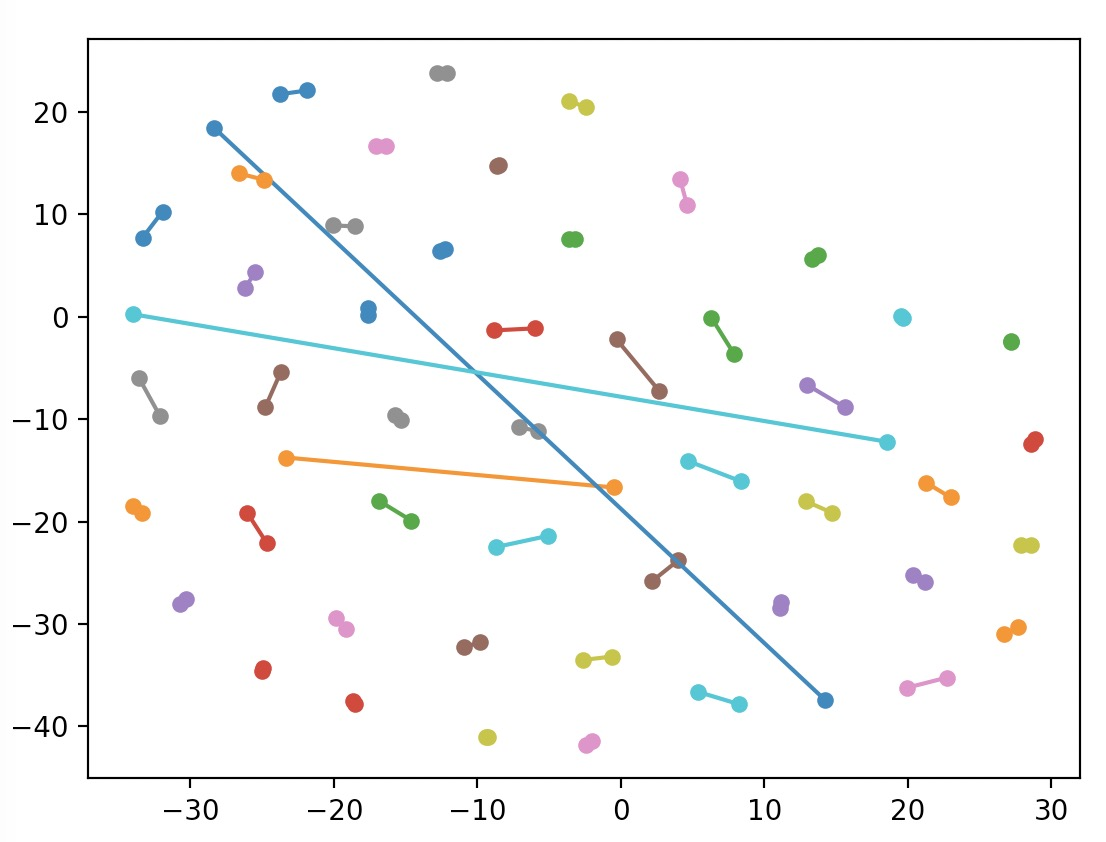
\includegraphics[width=\textwidth]{overlap}
    \caption{Perfect matching using maximum overlap of points in cluster}
    \label{fig:overlap}
  \end{subfigure}
  \begin{subfigure}[b]{0.5\textwidth}
    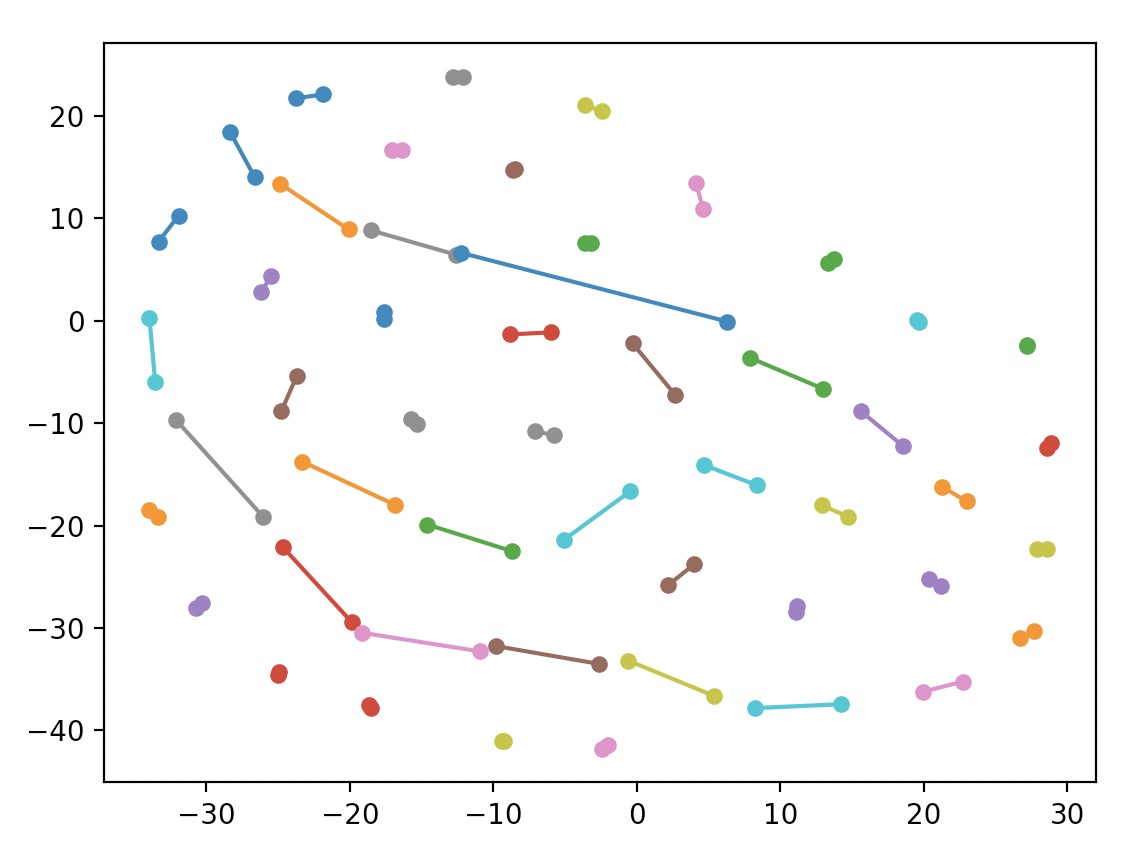
\includegraphics[width=\textwidth]{distance}
    \caption{Perfect matching using distances of cluster centres to each other.}
    \label{fig:distance}
  \end{subfigure}
  \caption{Example of different cost functions for perfect matching.}
\end{figure}

The figures \ref{fig:distance} and \ref{fig:overlap} are of cluster centres plotted in euclidean space. The axis are not labeled because it adds no extra information to our findings in this case. Every pairing of same-colour points on the plots come from $2$ different runs of the algorithm. We perfectly match the 100 points (50 per run), and get some interesting results.

Here we can see Figures ~\ref{fig:overlap} \& ~\ref{fig:distance} are very different even though they are run on the same datasets. There is a very good explanation for this that may not be clear at first glance. Figure ~\ref{fig:distances} seems to be inaccurate as there are clear pairings of points that weren't paired together. Rather than the closest points being paired, we see how there is a chain of pairings. This is because running the minimum weight perfect matching on the points based on Euclidean distance minimizes the overall distances between all the pairs, but does not take into consideration the actual underlying pairing that we are looking for.

In Figure \ref{fig:overlap}, maximum weight perfect matching of the centres is based on the number of shared points in the clusters. Here, we notice a very interesting pattern where the pairings seem to be near perfect overall with a few outliers that are far apart. While this is not exactly the expected result, it makes sense because for this dataset, we are not sure of the exact underlying number of clusters $k$. The real number of underlying clusters is likely to be lower than  $50$, the number inputted into the clustering run. The perfect matching makes that clear as some points are consistent over multiple runs while others seem to be completely random.

Through our experiments, it was clear that using the number of overlapping points of the clusters was a lot more effective in computing the perfect matching for our purposes. This raised the question if we are able to extract the real number $k$ of the underlying algorithm through a variant of this method. In the next chapter, we discuss our findings in that regard. 

\chapter{Determining the Number of Clusters $k$}
From our experiments and research, it was clear that inputting the incorrect number of clusters $k$ into the \kmeans algorithm, substantially affects performance, and accuracy. For that, we came up with an algorithm to help approximate the right number of clusters in the underlying dataset, before running the \kmeans algorithm.

The idea of the algorithm is relatively simple relying on the assumption that the real cluster centres of the underlying dataset will be present in most random runs of the algorithm, while the rest of the cluster centres will be relatively random based on the local area obtained through the initial seeding process. 

The algorithm takes a number which is the maximum number of clusters $k$ believed to be for the dataset, and the dataset. \kmeansn++ is run with the dataset $k$ times, and the centres produced are recorded. Then, we perfectly match centres from every unique pair of runs. Based on the matchings, we build a graph where every cluster centre in every run is a node that is connected to all the other nodes it was connected to by the matchings. Then we extract the number of disconnected components in the graph, and that tells us the estimated underlying number of clusters in the dataset. Because it is an estimate, running the above algorithm multiple times and taking the most frequent number is a heuristic that we found worked well.

The reason we believe this method works is because cluster centres that are accurate to the underlying dataset will be consistent in all the runs even if the inputted $k$ is not accurate. However, if the inputted $k$ is higher, then we will consistently get cluster centres that are somewhat random depending on how the algorithm was seeded. For that, in our experimental tests, we consistently had components of size $k$, while others had larger sizes. We believe that the components of size $k$ are the ones that are true for the underlying dataset.

Based on our experiments on a generated dataset, shown in Figure \ref{generatedDataset}, with $4$ clusters and $5,000$ per cluster, we were able to consistently get results between $3$ and $5$ for maxK input of $4$ to $9$. At maxK value of $10$, we got consistent results of $1$. This is a bit surprising, but makes sense because we can see how with a number $k$ that is higher than the real one in the underlying dataset will have a high probability of cluster centres matching to other components, grouping them all into one by the end.

\begin{figure}[h]
  \includegraphics[width=\textwidth]{generatedDataset}
  \caption{The generated dataset, $n=20,000 d=2$} 
  \label{fig:generatedDataset}
\end{figure}

The algorithm is still not perfect, but we believe that it can be fine-tuned with the different parameters to obtain a more accurate estimate of the number $k$. Another issue with the algorithm is running time, but that can be substantially improved with the introduction of multithreading and a few heuristics in the perfect matching step of the cluster centres. We believe this is an area of research worth more research.


\chapter{Extendable C++ Implementation}

Throughout the research for this paper, it was difficult to find modular code that is easily extendable for the \kmeans algorithm that allow us to perform testing on it. For that, we created our own implementation that is available on Github \footnote{The code is available at \url{https://github.com/technoligest/kmeansII}}.  This implementation is free to use and licenced under the MIT License.

The algorithm is implemented in highly optimized C++ with object-oriented programming at its core. This allows other developers to extend the algorithm and test different combinations of optimizations in the code. It can be used by both individuals needing to use a \kmeans implementation and ones who are looking to do research and optimize it further. 

Every \kmeans instance contains templated instances of a SeedPicker and an IterationRunner along with a skeleton that allows analysis of the performance of each run of the algorithm. This allows us to use different IterationRunners and SeedPickers interchangeably in the algorithm depending on the algorithm at hand and the resources allowed. The analytical data being saved at each run is independent of the SeedPicker and IterationRunner, which makes it simple for developers wanting to extend the algorithm.

The modularity of the implementation also allows developers to create new SeedPicker and IterationRunner classes. To create one, all they are required to do is implement a function from their respective Base class. For example, the $kd$-tree implementation of the algorithm has be hooked into a \kmeans instance by implementing it as an IterationRunner.



\chapter{Conclusion}

\kmeans is a method that has proven to be applicable to many domains and applications. It is still widely used. Unfortunately through rigorous testing, we have shown that the new \kmeansn-Consensus method of seeding the \kmeans algorithm is no better than randomly seeding the algorithm.



One area of research that is needed is a way to compute the real number $k$ for the algorithm. We have a method to compute that by calculating cliques in perfectly matched centres over multiple runs of the algorithm, but this needs further exploration. 


\bibliographystyle{newapa}
\bibliography{yaser_thesis}

\end{document}






% While \kmeans is widely used for its proven practical performance, it is not perfect for many use cases. The algorithm can give highly inaccurate clusters if the incorrect number $k$ is given to the algorithm. This is due to the nature of the algorithm forcing all the points into $k$ clusters. Another problem with the algorithm is that it produces convex shaped clusters, which inherently produces highly inaccurate clusters if the correct clusters are not convex shaped. The algorithm also struggles when there is a lot of noise\footnote{Note: Noise in this context is referring to the overlap of multiple clusters, where it becomes difficult to separate points if they are at the edges of two or more clusters.} in the data because having points between two clusters makes it difficult to force them into only one as membership becomes unclear. Inputting the incorrect number $k$ to the algorithm and/or having incorrect data leads to the algorithm struggling with running time and accuracy.